% =============================================================================
%  fig_relay_characteristic.tex
%  IEC Very-Inverse time-current characteristic curves (fixed vs adaptive)
%  plus instantaneous element threshold
% =============================================================================
\documentclass[tikz, border=8pt]{standalone}
\usepackage{tikz}
\usepackage{pgfplots}
\pgfplotsset{compat=1.18}
\usepackage{amsmath}

\begin{document}
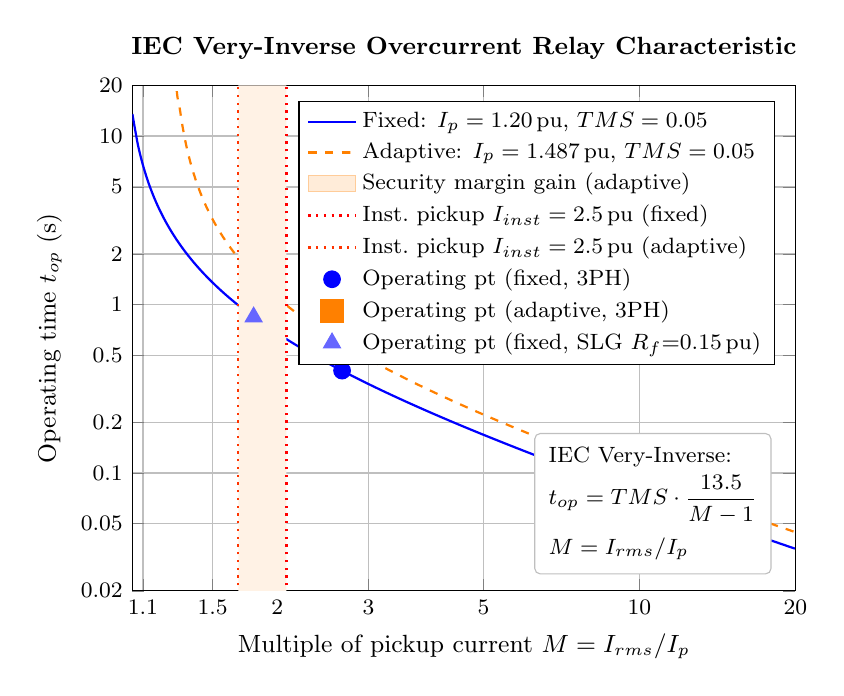
\begin{tikzpicture}
\begin{loglogaxis}[
  width     = 10cm,
  height    = 8cm,
  xmin=1.05, xmax=20,
  ymin=0.02, ymax=20,
  xlabel    = {Multiple of pickup current $M = I_{rms}/I_p$},
  ylabel    = {Operating time $t_{op}$ (s)},
  title     = {IEC Very-Inverse Overcurrent Relay Characteristic},
  grid      = both,
  grid style= {line width=0.3pt, gray!30},
  major grid style = {line width=0.5pt, gray!50},
  xtick     = {1.1, 1.5, 2, 3, 5, 10, 20},
  xticklabels = {1.1, 1.5, 2, 3, 5, 10, 20},
  ytick     = {0.02, 0.05, 0.1, 0.2, 0.5, 1, 2, 5, 10, 20},
  yticklabels= {0.02, 0.05, 0.1, 0.2, 0.5, 1, 2, 5, 10, 20},
  legend pos = north east,
  legend style = {font=\footnotesize, cells={anchor=west}},
  label style = {font=\small},
  tick label style={font=\footnotesize},
  title style= {font=\small\bfseries},
  clip      = true,
]

% ---- IEC Very-Inverse: t = TMS * (13.5 / (M-1)) ----------------------------

% Fixed relay: Ip=1.20, TMS=0.05  => t = 0.05 * 13.5/(M-1)
\addplot[blue, thick, domain=1.05:20, samples=120, smooth]
  {0.05 * 13.5 / (x - 1.0)};
\addlegendentry{Fixed: $I_p=1.20$\,pu, $TMS=0.05$}

% Adaptive relay: Ip=1.487, TMS=0.05
% On the fixed M-axis: M_adapt = M_fixed * (1.20/1.487) = M_fixed * 0.8071
% => t = 0.05 * 13.5 / (M*0.8071 - 1)  — curve shifts right (needs more current to trip)
\addplot[orange, thick, dashed, domain=1.24:20, samples=120, smooth]
  {0.05 * 13.5 / (x * 0.8071 - 1.0)};
\addlegendentry{Adaptive: $I_p=1.487$\,pu, $TMS=0.05$}

% ---- Shaded region: adaptive discriminates better (drawn before markers) ----
\addplot[fill=orange!10, draw=none, forget plot]
  coordinates {(1.682, 0.02)(2.083, 0.02)(2.083,20)(1.682,20)} \closedcycle;
\addlegendimage{area legend, fill=orange!15, draw=orange!40}
\addlegendentry{Security margin gain (adaptive)}

% ---- Instantaneous element: Iinst=2.5 pu -----------------------------------
% In M-units for fixed relay: M_inst = 2.5/1.20 = 2.083
\addplot[red, thick, dotted]
  coordinates {(2.083, 0.001) (2.083, 20)};
\addlegendentry{Inst.\ pickup $I_{inst}=2.5$\,pu (fixed)}

% Adaptive instantaneous: 2.5/1.487 = 1.682
\addplot[red!60!orange, thick, dotted]
  coordinates {(1.682, 0.001) (1.682, 20)};
\addlegendentry{Inst.\ pickup $I_{inst}=2.5$\,pu (adaptive)}

% ---- Operating points -------------------------------------------------------
% 3PH fault: I_rms ≈ 3.2 pu
% Fixed:    M = 3.2/1.20 = 2.667, t = 0.05*13.5/1.667 = 0.405 s
% Adaptive: M_fixed = 2.667, t_adapt = 0.05*13.5/(2.667*0.8071-1) = 0.05*13.5/1.152 = 0.586 s
\addplot[blue, only marks, mark=*, mark size=3pt]
  coordinates {(2.667, 0.4054)};
\addlegendentry{Operating pt (fixed, 3PH)}

\addplot[orange, only marks, mark=square*, mark size=4pt]
  coordinates {(2.667, 0.5859)};
\addlegendentry{Operating pt (adaptive, 3PH)}

% SLG fault: mid-level, M=1.8 for fixed, t = 0.05*13.5/0.8 = 0.844 s
\addplot[blue!60, only marks, mark=triangle*, mark size=3.5pt]
  coordinates {(1.8, 0.844)};
\addlegendentry{Operating pt (fixed, SLG $R_f{=}0.15$\,pu)}

% ---- Characteristic equation annotation — lower right, clear of legend ------
\node[draw=gray!50, fill=white, rounded corners=2pt, inner sep=5pt,
      align=left, font=\footnotesize, anchor=south east]
  at (axis cs: 18, 0.025)
  {IEC Very-Inverse:\\[2pt]
   $\displaystyle t_{op} = TMS \cdot \dfrac{13.5}{M - 1}$\\[4pt]
   $M = I_{rms} / I_p$};

\end{loglogaxis}
\end{tikzpicture}
\end{document}
